\documentclass{template}
\title{Summary - Probability Theory}

\newcommand{\Poisson}{\text{Poisson}}
\newcommand{\Binomial}{\text{Bin}}

\begin{document}
\maketitle

\section{Distributions}

\subsection{Concepts}

\subsubsection{Percentile}
Let $p$ be a number between 0 and 1, the $100p$-th percentile of a rv $X$
denoted by $\eta(p)$ is defined by
\[
	P(X \leq \eta(p)) = p
\] 
or equivalently,
\[
	p = F(\eta(p)) = \int_{-\infty}^{\eta(p)} f(x) dx
\] 
\subsubsection{Critical Value of Standard Normal Distribution}
$z_\alpha$ is defined by $P(Z \geq z_\alpha) = \alpha$

In other words, $z_\alpha$ is the $100(1-\alpha)$-th percentile of the standard normal distribution.

\begin{center}
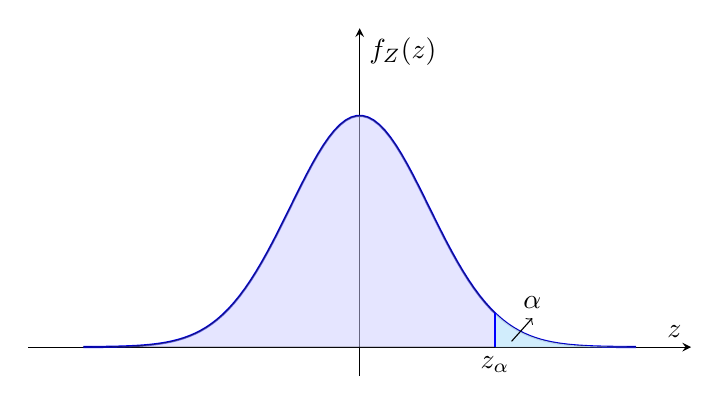
\begin{tikzpicture}
	\begin{axis}[
		xmin=-4, xmax=4,
		ymin=0, ymax=0.5,
		axis lines=middle,
		enlargelimits,
		ticks=none,
		width=10cm,
		height=6cm,
		domain=-4:4,
		samples=100,
		ylabel={$f_Z(z)$},
		xlabel={$z$},
	]
	\addplot[blue, thick] {1/sqrt(2*pi) * exp(-x^2/2)};
	\addplot[fill=blue!20, opacity=0.5] {1/sqrt(2*pi) * exp(-x^2/2)} \closedcycle;
	% fill the area to the right of z_alpha
	\addplot[
			fill=cyan!20, opacity=0.8,
			draw=none,
			domain=1.96:4,
			samples=200
	] {1/sqrt(2*pi) * exp(-x^2/2)} \closedcycle;

	\draw[blue,thick] (axis cs: 1.96,0) -- (axis cs: 1.96,{1/sqrt(2*pi) * exp(-1.96^2/2)});
	
	\node at (axis cs: 1.96, 0) [below] {$z_\alpha$};
	\draw[->] (axis cs: 2.2, 0.01) -- (axis cs: 2.5, 0.05) node[above] {$\alpha$};
	\end{axis}
\end{tikzpicture}
\end{center}

\subsection{Binomial Distribution}
Binomial distribution is denoted by \( \Binomial(n, p) \), where \( n \) is the number of trials and \( p \) is the probability of success in each trial. The random variable \( X \) represents the number of successes in \( n \) independent Bernoulli trials.
PMF is given by
\[
	P(X=k) = \binom{n}{k} p^k (1-p)^{n-k}, \quad k=0,1,2,\ldots,n
\]
the expected value is $np$
\begin{proof}
	Let $Y_k$ be the indicator random variable for the $k$-th trial, which takes the
	value 1 if the $k$-th trial is a success and 0 otherwise. Then,
	 \[
		E[Y_k] = 1 \cdot P(Y_k=1) + 0 \cdot P(Y_k=0) = p
	\] 
	by the independence,
	\[
		E[X] = E\left[\sum_{k=1}^{n} Y_k\right] = \sum_{k=1}^{n} E[Y_k] = np
	\] 
\end{proof}
the variance is $np(1-p)$
\begin{proof}
	\[
		E[Y_k^2] = 1^2 \cdot P(Y_k=1) + 0^2 \cdot P(Y_k=0) = p
	\] 
	\[
		V[Y_k] = E[Y_k^2] - E[Y_k]^2 = p - p^2 = p(1-p)
	\] 
	by the independence,
	\[
		V[X] = V\left[\sum_{k=1}^{n} Y_k\right] = \sum_{k=1}^{n} V[Y_k] = np(1-p)
	\] 
\end{proof}

\subsection{Poisson Distribution}
Poisson distribution is denoted by \( \Poisson(\mu) \), or $P(\mu)$, where
 \( \mu \) is the average number of events in a fixed interval of time or space.
If the expected number of events in a given interval time length $t$ is $\lambda$
then $\mu=\lambda t$.
The random variable \( X \) represents the number of events occurring in that interval.
PMF is given by
\[
	P(X=k) = \frac{\mu^k e^{-\mu}}{k!}, \quad k=0,1,2,\ldots
\] 
The expected value and variance of Poisson distribution are both equal to \( \mu \)
\begin{proof}
\[
	E[X] = \mu e^{-\mu}\sum_{k=1}^{\infty} \frac{\mu^{k-1} }{(k-1)!} = 
	\mu e^{-\mu} e^{\mu} = \mu
\] 
\[
	E[X^2] = \mu e^{-\mu}\sum_{k=1}^{\infty} \frac{k-1+1}{(k-1)!} \mu^{k-1}
	= \mu e^{-\mu} \left( 
	\mu\sum_{k=2}^{\infty} \frac{\mu^{k-2}}{(k-2)!} + e^{\mu} \right)
	= \mu^2 + \mu
\] 
\[
	V[X] = E[X^2] - E[X]^2 = \mu
\] 
\end{proof}

\subsubsection{Relationship between Binomial and Poisson Distributions}
The Poisson distribution can be derived as a limiting case of the Binomial 
distribution when \( n \to \infty \) and \( p \to 0 \) such that \( np = \mu \) remains
constant. 
Meaning, we cut the time interval into \( n \) subintervals, and let \( p \) be the probability
of an event occurring in each subinterval, while keeping the expected number of events
$np$ equal to original average $\lambda t$.
In this case,
\[
	\begin{aligned}
		P(X=k) &= \lim_{n \to \infty} \frac{n!}{k!(n-k)!} \left(\frac{p}{1-p}\right)^k
		((1-p)^{1/p})^{np}\\
					 &= \lim_{n \to \infty} \frac{n(n-1)\cdots(n-k+1)}{k!} p^k e^{-np}\\
					 &= \lim_{n \to \infty} \frac{n^k}{k!} p^k e^{-\mu}
					 = \frac{\mu^k e^{-\mu}}{k!}
	\end{aligned}
\] 


\subsection{Hypergeometric Distribution}
The hypergeometric rv \( X \) represents the number of successes in \( n \) draws
without replacement from a finite population of size \( N \) that contains
exactly \( M \) successes. The PMF is given by
\[
	P(X=k) = \frac{\binom{M}{k}\binom{N-M}{n-k}}{\binom{N}{n}}, \quad k=0,1,2,\ldots,n
\] 
the expected value is \( n\frac{M}{N} \)
and the variance is
\[
	V[X] = \frac{N-n}{N-1} n \frac{M}{N} \left(1-\frac{M}{N}\right)
\] 
\begin{remark}
	If let \( p = \frac{M}{N} \) be the probability of success in a single draw, then
	the expected value is the same as the Binomial distribution, while the variance
	is smaller than the Binomial distribution by a factor of \( \frac{N-n}{N-1} \).
\end{remark}

\subsection{Negative Binomial Distribution}
The negative binomial rv \( X \) represents the number of trials needed to achieve
exactly \( r \) th successes in a sequence of independent Bernoulli trials with
probability of success \( p \). The PMF is given by
\[
	P(X=k) = \binom{k-1}{r-1} p^r (1-p)^{k-r}, \quad k=r,r+1,r+2,\ldots
\] 
The expected value is \( \frac{r}{p} \)
and the variance is \( \frac{r(1-p)}{p^2} \)
\subsection{Normal Distribution}
Normal distribution is denoted by \( N(\mu, \sigma^2) \), where \( \mu \) is the mean and \( \sigma^2 \) is the variance.
The PDF is given by
\[
	f(x) = \frac{1}{\sigma \sqrt{2\pi}} e^{-\frac{(x-\mu)^2}{2\sigma^2}},\quad -\infty < x < \infty
\]
\begin{proof}
	\[
		E[X] = \frac{1}{\sigma \sqrt{2\pi}} \int_{-\infty}^{\infty} (x-\mu) e^{-\frac{(x-\mu)^2}{2\sigma^2}} dx
		+ \frac{\mu}{\sigma \sqrt{2\pi}} \int_{-\infty}^{\infty} e^{-\frac{(x-\mu)^2}{2\sigma^2}} dx
		= 0 + \mu = \mu
	\] 
	\[
		V[X] = \frac{1}{\sigma \sqrt{2\pi}} \int_{-\infty}^{\infty} t^2 e^{-\frac{t^2}{2\sigma^2}} dt
		= \frac{1}{\sigma \sqrt{2\pi}} \int -\sigma^2 t \dd e^{-\frac{t^2}{2\sigma^2}} 
		= -\frac{\sigma}{\sqrt{2\pi}} \left[ t e^{-\frac{t^2}{2\sigma^2}} \right]_{-\infty}^{\infty} 
		+ \frac{\sigma}{\sqrt{2\pi}} \int_{-\infty}^{\infty} e^{-\frac{t^2}{2\sigma^2}} dt
		= 0 + \sigma^2 = \sigma^2
	\] 
\end{proof}

\subsubsection{Linearity of Normal Distribution}
Given two \textbf{independent} normal random variables \( X \sim N(\mu_1, \sigma_1^2) \) and 
\( Y \sim N(\mu_2, \sigma_2^2) \), the linear combination \( Z = aX + bY + c \) is
also normally distributed, with mean \( a\mu_1 + b\mu_2 + c \) and variance \( a^2\sigma_1^2 + b^2\sigma_2^2 \).

\subsection{Uniform Distribution}
The uniform distribution rv \( X \) in the interval \( [A, B] \) 
has
\[
	E[X] = \frac{A+B}{2}, \quad V[X] = \frac{(B-A)^2}{12}
\] 
\subsection{Exponential Distribution}
The exponential distribution rv \( X \) with rate parameter \( \lambda > 0 \) has
PDF
\[
	f(x) = \lambda e^{-\lambda x}, \quad x \geq 0
\] 
with
\[
	E[X] = \frac{1}{\lambda}, \quad V[X] = \frac{1}{\lambda^2}
\] 
\begin{proof}
	\[
		E[X] = \int_{0}^{\infty} x \lambda e^{-\lambda x} dx
		= -x e^{-\lambda x} \Big|_{0}^{\infty} + \int_{0}^{\infty} e^{-\lambda x} dx
		= 0 + \frac{1}{\lambda} = \frac{1}{\lambda}
	\] 
	\[
		E[X^2] = \int_{0}^{\infty} x^2 \lambda e^{-\lambda x} dx
		= -x^2 e^{-\lambda x} \Big|_{0}^{\infty} + 2 \int_{0}^{\infty} x e^{-\lambda x} dx
		= 0 + 2 \cdot \frac{1}{\lambda^2} = \frac{2}{\lambda^2}
	\] 
	\[
		V[X] = E[X^2] - E[X]^2 = \frac{2}{\lambda^2} - \frac{1}{\lambda^2} = \frac{1}{\lambda^2}
	\] 
\end{proof}

\subsubsection{Relationship between Exponential and Poisson Distributions}
The exponential distribution can describe the time between events in a Poisson
process. Let $T$ denotes the time until the first event occurs(equivalently to the time between events
according to the time-homogeneous property of Poisson process), then the CDF of $T$ is
\[
	F_T(t) = 1-P(T > t) = 1-P(0 \text{ events occur in } [0, t]) = 1-P_{\Poisson}(X=0) = 1-e^{-\mu} 
	= 1-e^{-\lambda t}
\] 
Taking the derivative of the CDF, we get the PDF of $T$:
\[
	f_T(t) = \frac{d}{dt} F_T(t) = \lambda e^{-\lambda t}, \quad t \geq 0
\] 

\section{Transformations of Random Variables}

Given a random variable \( X \) with PDF \( f_X(x) \), and a transformation
\(Y = g(X) \), and we want to find the PDF of \( Y \), denoted by \( f_Y(y) \).

A common method is to use CDF transformation. Let \( F_X(x) \) be the CDF of \( X \), then
the CDF of \( Y \) is given by solving the inequality
\[
	F_Y(y) = P(Y \leq y) = P(g(X) \leq y) 
\] 
and if \( g \) is a invertible and monotonic function, we can use so called
Jacobian/change of variable method. Let \( h = g^{-1} \) be the inverse function of \( g \), then
\[
	f_Y(y) = f_X(h(y)) \left| \frac{dh(y)}{dy} \right|
\] 

\end{document}
